\chapter*{Abstract}
\textcolor{red}{Work in progress}\\
As technology grows, the amount of devices that are part of our daily life rises as well. Since childhood, the new generations are learning to interact with technology while playing with new games implemented in embedded systems. This phenomenon can be seen on a large scale with robot games. New researches are made on robots developed to interact with human players in a game environment. Games not only make people have fun, but they are one of the most powerful tools for socialization, and cognitive development~\cite{vygotsky_play_1967, sylva_play:_1976, piaget_play_2013}.  While playing competitive games, a person is encouraged to learn the opponent's behavior for various reasons; for example, having a good knowledge of the opponent's behavior is essential for building a winning strategy, and this plays an important role in creating amusement.

%\begin{figure}[htbp]
%\centerline{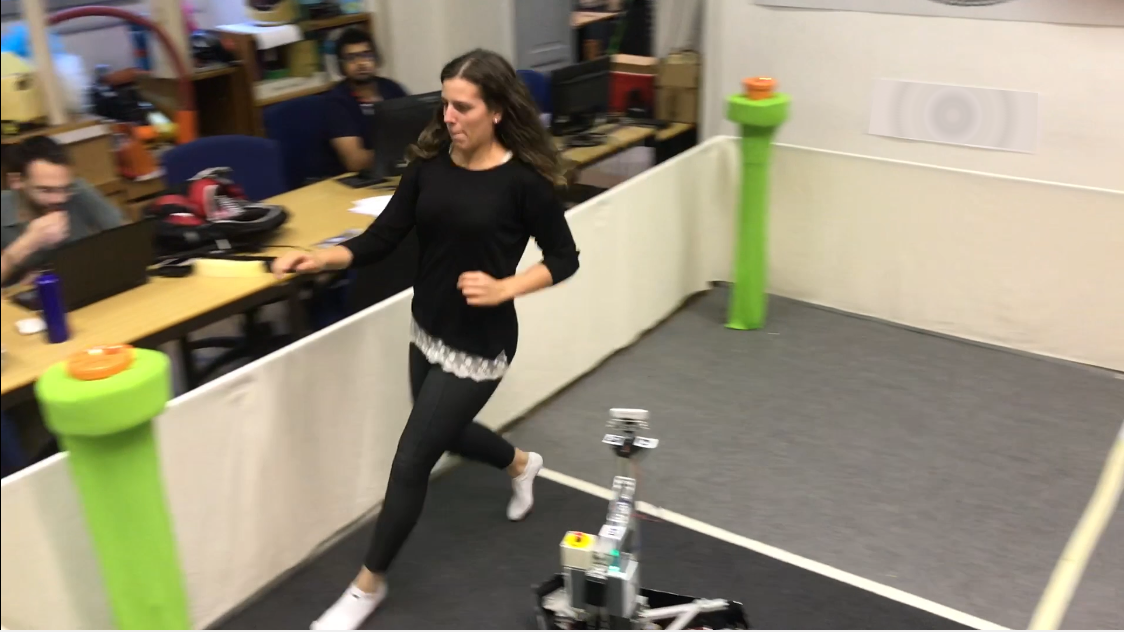
\includegraphics[width=0.5\columnwidth]{images/06-deception/frontPaper23}}
%\caption{Human-Robot interaction scene from our experiments.}
%\label{fig::front}
%\end{figure}

The main issues that should be faced in this field concern the robot's intelligence as perceived by the human player: low or too high levels may induce the player to leave because the robot is not considered as a valid competitor, and this lowers the entertainment level of the game. 

We are focusing on a challenging type of games, where the players are involved in a physical, quite demanding activity. This type of games has been introduced as~\gls{pirg}~\cite{martinoia_physically_2013}). In~\gls{pirg}s, it is important to model the player, by using the only available data that could describe well enough the movements of the player.